\documentclass[slidestop,compress,mathserif,note=show, blackandwhite]{beamer}
%% [slidestop] puts frame titles on the top left corner
%% (default=[slidescentered]).
%% [compress] makes all navigation bars as small as possible
%% (default=[uncompressed]).
%% [red] changes navigation bars and titles to reddish color.

\usepackage{graphics}

% for bold faced structures (titles, headlines, footlines, sidebars, ...)
\usefonttheme{structurebold}



\definecolor{myYellow}{RGB}{252,187,6}

%hideallsubsections, hideothersubsections
\usetheme[left]{Goettingen}                  % Beamer theme v 3.0
\usecolortheme{crane}                % Beamer color theme

\setbeamercolor{title}{fg=black}
\setbeamercolor{frametitle}{fg=black}
\setbeamercolor{section in sidebar}{fg=black, bg=myYellow}
\setbeamercolor{section in sidebar shaded}{fg=blue}
\setbeamercolor{subsection in sidebar}{fg=black, bg=myYellow}
\setbeamercolor{subsection in sidebar shaded}{fg=black}

% general data
\title [R.E.A.R.] {Rear Exocentric Augmented Reality}
\subtitle []{an exocentric vision framework for mobile robot teleoperations}
\author []{Daniele Ferro}
\date []{March 29, 2011}
\institute [UniCT] {Universit\`a di Catania\\Dipartimento di Ingegneria Elettrica Elettronica e Informatica [DIEEI]}

\begin{document}

% Cover slide
\begin{frame}    
 \titlepage
\end{frame}

% slide indice
\section[Outline]{}
%\tiny
\frame{

  \frametitle{Outline}
  \tableofcontents
}
\small

%% INTRODUCTION %%

\section{Introduction}
\subsection{Teleoperation \& telepresence}
\frame
{
  \frametitle{Teleoperation \& telepresence}
  
  \textit{we need the equivalent of a body in a remote environment,
    with which we can move around, perform the proper actions through,
    observe with.}

  \pause

  \begin{itemize}
    
    \item \textit{teleoperation} \\
      doing work at distance
      \pause

    \item \textit{telepresence} \\
      feeling like you are somewhere else

  \end{itemize}
  
}

\subsection{The 3m.o.r.d.u.c. platform}
\frame
{
  \frametitle{The  3m.o.r.d.u.c. platform}
  
  \begin{center}
    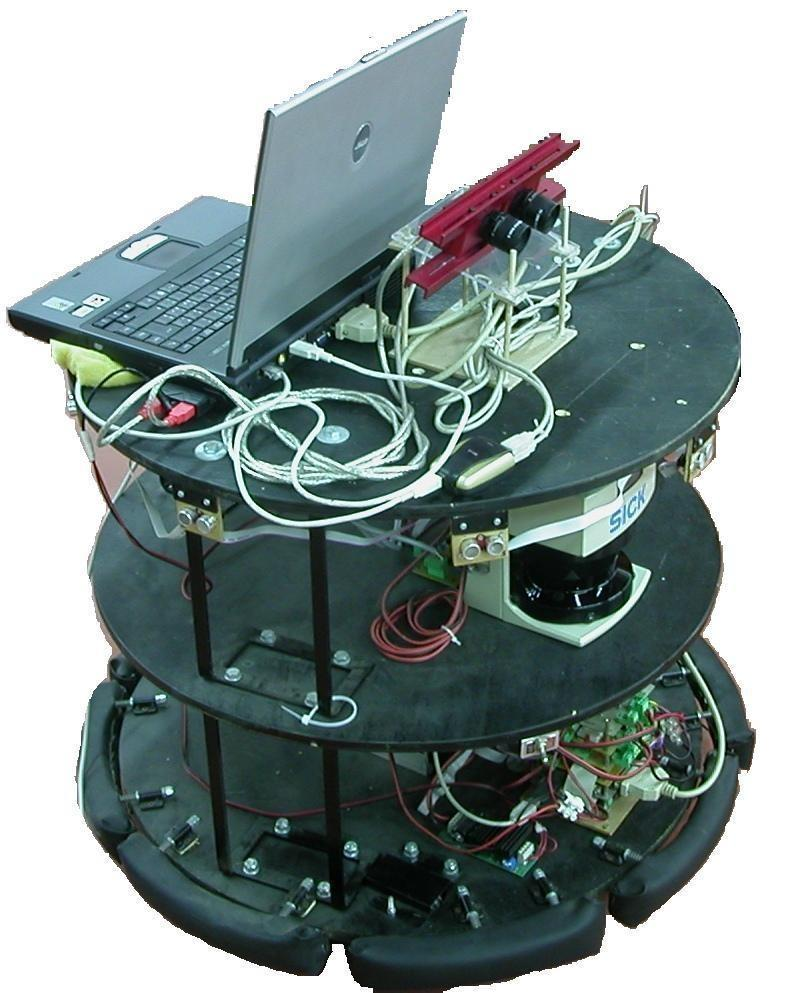
\includegraphics[height=3cm]{img/3morduc.jpg}
  \end{center}
  
  Main features: \\
  \pause

  \begin{itemize}
    
    \item \textit{mobility configuration} \\
      differential-drive
      \pause

    \item \textit{sensors} \\
      encoders, sonar, laser, bumpers, stereocameras
      \pause

    \item \textit{communication protocol} \\
      HTTP server

  \end{itemize}
  
}


%% EXOCENTRIC VISION

\section{The exocentric vision}
\subsection{Why exocentric vision ?}
\frame
{
  \frametitle{Why exocentric vision ?}
  \textit{it's difficult for an operator not accustomed to the vehicle
    to estimate the vehicle's position and direction and the distances to a target strictly
    based on camera images from the first person viewpoint.}
  \pause
  \vspace {1.0cm}
 
  \textcolor{red}{\texttt{Idea}}: an exocentric camera would provide a view of the robot in the operating
  environment and, thus, a better understanding of where the robot is located into the
  environment and its actual direction. \\
  \pause
  \vspace {1.0cm}
  
  \textcolor{red}{\texttt{Contr}}: exocentric camera could be mounted on a rear-mounted protuberance of the robot,
  but such a protuberance would terribly limit the robot activity and its moving abilities.
  \pause
  \vspace {1.0cm}

  \textcolor{red}{\texttt[color=red]{Solution}}: simulate a virtual exocentric point of view by means of previous egocentric
  images.

}


\section{Log data}

\section{R.E.A.R.}

\section{Exocentric vision for 3morduc}



\end{document}
